\documentclass{article}
\usepackage{graphicx}
\usepackage[margin=1.5  in]{geometry}
\hyphenation{contributed insightful inputs practical understanding comprehensive Niraula supervisor enriching discussions willingness acknowledge}
\begin{document}

\pagenumbering{roman}

\newpage

\begin{center}
	\thispagestyle{empty}
	\large\textbf{TRIBHUVAN UNIVERSITY}\\
	\large\textbf{INSTITUTE OF ENGINEERING }\\
	\vspace{0.1in}
	\LARGE{\textbf{Khwopa College Of Engineering}\\}
	\vspace{0.1cm}
%	\normalsize{Libali, Bhaktapur\\}
	\large\textbf{Department of Computer Engineering}
	\vspace{0.4in}
	\begin{figure}[h]
			\centering
				
\includegraphics[width=0.3\textwidth]{img/Khwopalogo.jpg}
	\end{figure}
	
	\vspace{0.4in}
	\large{\textbf{A REPORT ON}\\Instrumentation-II Case Study\\}
	
	\vspace{0.5in}
%	\large{\textit{Submitted in partial fulfillment of the requirements for the degree\\}}
	
%	\large{\textbf{BACHELOR OF COMPUTER ENGINEERING}\\}
	
	\large{\textbf{Visit Undertaken at}\\}
		\normalsize{Gorkha Eco Red Bricks Company Pvt. Ltd.\\
			Mahendrajyoti, Nepal\\
		}
		\vspace{0.5in}
	\large{\textbf{Submitted by:}}\\
	\vspace{0.2cm}
	\begin{tabular}{p{2in}p{1.2in}}
		\hspace{0.3cm}Manish Pyakurel & KCE077BCT020\\
		\hspace{0.3cm}Rupak Neupane & KCE077BCT028\\
		\hspace{0.3cm}Sarjyant Shrestha & KCE077BCT033\\
		\hspace{0.3cm}Srijan Gyawali & KCE077BCT036\\
	 \vspace{0.2in}
	\end{tabular}
	\\
%	\vspace{0.5cm}
%	\large{\textbf{Under the Supervision of}\\}
%		\normalsize{Er.Dinesh Gothe\\
%			Department Of Computer Engineering\\
%		}
		\vspace{0.4in}
		\normalsize{Libali, Bhaktapur\\
		2023-08-24	
	}
\end{center}


  
% acknowledgement.tex
\begin{center}
\section*{Acknowledgment}
\end{center}
\addcontentsline{toc}{section}{Acknowledgment}
I would like to express my heartfelt gratitude to the individuals who have contributed to the successful completion of the case study on Instrumentation II, focusing on the Gorkha Eco Red Bricks process.
\vspace{0.4cm} \\
First and foremost, I extend my sincere thanks to Er. Dinesh Gothe, Head of the Department, for his invaluable guidance, unwavering support, and insightful inputs throughout this case study. Your expertise and encouragement have been instrumental in shaping our understanding of the subject matter.
I am also deeply appreciative of the efforts and dedication shown by Ms. Ekata Niraula, our esteemed lecturer. Your thorough explanations, thought-provoking discussions, and willingness to address our queries have been pivotal in enriching our knowledge and driving this case study towards excellence.
I extend a special note of appreciation to Mr. Mesun Lakhemaru, our field supervisor, whose practical insights and real-world experience have provided us with a comprehensive understanding of the Gorkha Red Bricks process. Your willingness to share your expertise and guide us through practical intricacies is genuinely commendable.
\vspace{0.4cm} \\
I would like to express my gratitude to the entire academic community for fostering an environment of learning and exploration. Your collective efforts have played a significant role in our academic growth.
Lastly, I would like to acknowledge the support of my fellow classmates and colleagues who have shared ideas, experiences, and resources, contributing to the overall quality of this case study.


\newpage

\tableofcontents
\addcontentsline{toc}{section}{Table of Contents}

\newpage
\pagenumbering{arabic}

\section{Introduction}
% Your introduction content goes here.

\subsection{About Organization}
After a dedicated and focused effort spanning a year and a half, Gorkha Red Brick Pvt. Ltd. has celebrated a significant achievement in the form of the newly launched product "Gorkha Chinese Itta." This accomplishment stands as a testament to their commitment to innovation within Nepal's brick-making industry. Brick production is deeply embedded in Nepal's cultural heritage. Bricks have been an essential building material, especially in regions near the Kathmandu Valley. In this context, Gorkha Red Brick's recent accomplishment signifies a meaningful progression in the tradition of brick manufacturing.

\vspace{0.4cm}
What truly sets Gorkha Red Brick apart is their embrace of modern technology. The introduction of Tunnel Kiln Technology represents a groundbreaking advancement in brick production. With an impressive daily capacity of 100,000 bricks, this cutting-edge approach has revolutionized the manufacturing process.
The operation of Tunnel Kiln involves three distinct zones. In the preheating phase, the bricks receive initial warmth. The firing phase, which occurs in the central part of the tunnel, is where the transformation takes place. Finally, the cooling zone ensures the bricks are prepared for use.
While the technology is undeniably advanced, its eco-friendliness is equally noteworthy. Gorkha Red Brick's commitment to environmental sustainability is evident in their choice of energy-efficient methods. By prioritizing this approach, they are not only meeting market demands but also contributing positively to the environment.

\vspace{0.4cm}
Gorkha Red Brick's journey to this achievement has been guided by a clear vision. Their focus on innovation is a reflection of their determination to evolve beyond traditional brick-making practices. In successfully bridging the gap between tradition and modernity, they have not only created a superior product but also illuminated a pathway for the industry's future.
This accomplishment speaks volumes about Gorkha Red Brick's value as a forward-looking enterprise. Their achievement extends beyond bricks, serving as an embodiment of progress and responsible production. With every brick produced using the Tunnel Kiln Technology, they are shaping a future that is not only promising but also sustainable.

\newpage
\subsection{Composition of bricks: Function of ingredients}
Bricks are rectangular units of construction material. Bricks are used in masonry construction, walls, and pavements. It is used as a substitute of stone, where the stone is not readily available. Brick chips are often used as coarse aggregate in the concrete mix.
Percentage of Constituents of Brick (Weight Basis).
There are six major ingredients of brick. The general percentage of these ingredients in brick is given below:\\
Ingredient	Percentage in brick
Silica (SiO2)	55\%\\
Alumina (Al2O3)	30\%\\
Iron Oxide (Fe2O3)	8\%\\
Magnesia (MgO)	5\%\\
Lime(CaO)	1\%\\
Organic Matter	1\%\\
\vspace{0.1cm}\\
Chief Ingredients of Brick and Their Functions
Silica (Sand) and Alumina (Clay), these two are the most prominent ingredients in brick clay. When mixed with water in proper proportions, it gains plasticity. The plastic mass can be easily molded and dried. It should not go through cracking, shrinkage or warping.\\
\vspace{0.1cm}\\
Alumina\\
Alumina is the main constituent of clay. It acts as a cementing material in raw brick. Brick clay is plastic due to the presence of alumina. This plasticity ensures that bricks can be molded. An excess amount of alumina in clay may cause the bricks to shrink, warp or crack on drying and burning as any other cementing material.\\
\vspace{0.1cm}\\
Silica\\
Good quality bricks contain 50-60\% silica. It is present in both free and combined form. As frees sand, it remains mechanically mixed with clay. In combined form, it reacts with alumina to form aluminosilicates. Silica prevents raw bricks from cracking, shrinking and warping. The higher the proportion of sand, the more and shapely and uniform in texture will be the brick. Although, excess silica destroys cohesion between the brick clay particles and makes brick brittle and weak. The durability of bricks largely depends upon the proper proportion of silica and alumina.\\
\vspace{0.1cm}\\
Lime\\
Bricks should contain a little amount of finely powdered lime. It enables silica (of a required portion) to melt at the furnace temperature of 1650oC and binds the particles of brick together resulting in strong and durable bricks. At about 1100 degC, lime acts as a catalyst to elevate the furnace temperature to 1650oC at which silica fuses. This slightly fused silica works as a strong cementing material. Excess lime in brick clay will cause vitrification of bricks. It causes bricks to melt, as more than the required amount of silica will fuse. The bricks then lose their shape and become disfigured.\\
\vspace{0.1cm}\\
Iron Oxide\\
Bricks contain a small quantity of Iron Oxide. Iron Oxide acts a flux like lime, thus helps silica to fuse at low temperature. It imparts a red color to bricks upon burning. Iron also increases the durability and impermeability of the bricks.\\
\vspace{0.1cm}\\
Magnesia\\
A small proportion of magnesium decreases shrinkage and gives a yellow tint to the bricks. An excess amount of it causes bricks to decay.\\
\vspace{0.1cm}\\
Harmful Ingredients of Brick\\
Lime\\
Excess lime melts the bricks and disfigures it. If CaCO3 exists (in the purest form, i.e., if it contains at least 95\% CaO) in lime-lump in brick clay, it converts into quicklime on burning. When these bricks come in contact with water, quicklime slakes and expands. And causes disintegration of bricks.\\
\vspace{0.1cm}\\
Alkalis\\
Alkalis are mainly salt of Sodium (Na) and Potassium (K). It acts as a flux in the kiln and causes fusion, warping, and twisting of bricks. Alkalis absorb moisture from the atmosphere and cause dampness and efflorescence in bricks (because of the presence of hygroscopic salts, e.g., CaCl2, MgCl2, etc.).\\
\vspace{0.1cm}\\
Pebbles, Stones and Gravels\\
Their presence does not allow thorough mixing of earth, thus the bricks produced are weaker. Such bricks cannot be broken at the desired section and they break very irregularly.\\
\vspace{0.1cm}\\
Iron Pyrites (FeS)\\
Iron Pyrites causes crystallization and disintegration of bricks while burning. It discolors bricks in the form of black slag.\\
\vspace{0.1cm}\\
Organic Matter\\
Organic matter in bricks makes bricks porous resulting in low density and weaker bricks production.\\

\newpage
\section{Brick Manufacturing Process}
% Information about the manufacturing process of bricks.

\subsection{Block Diagram}
% Description of the block diagram of the brick manufacturing process.
\begin{figure}[h]
  \centering
  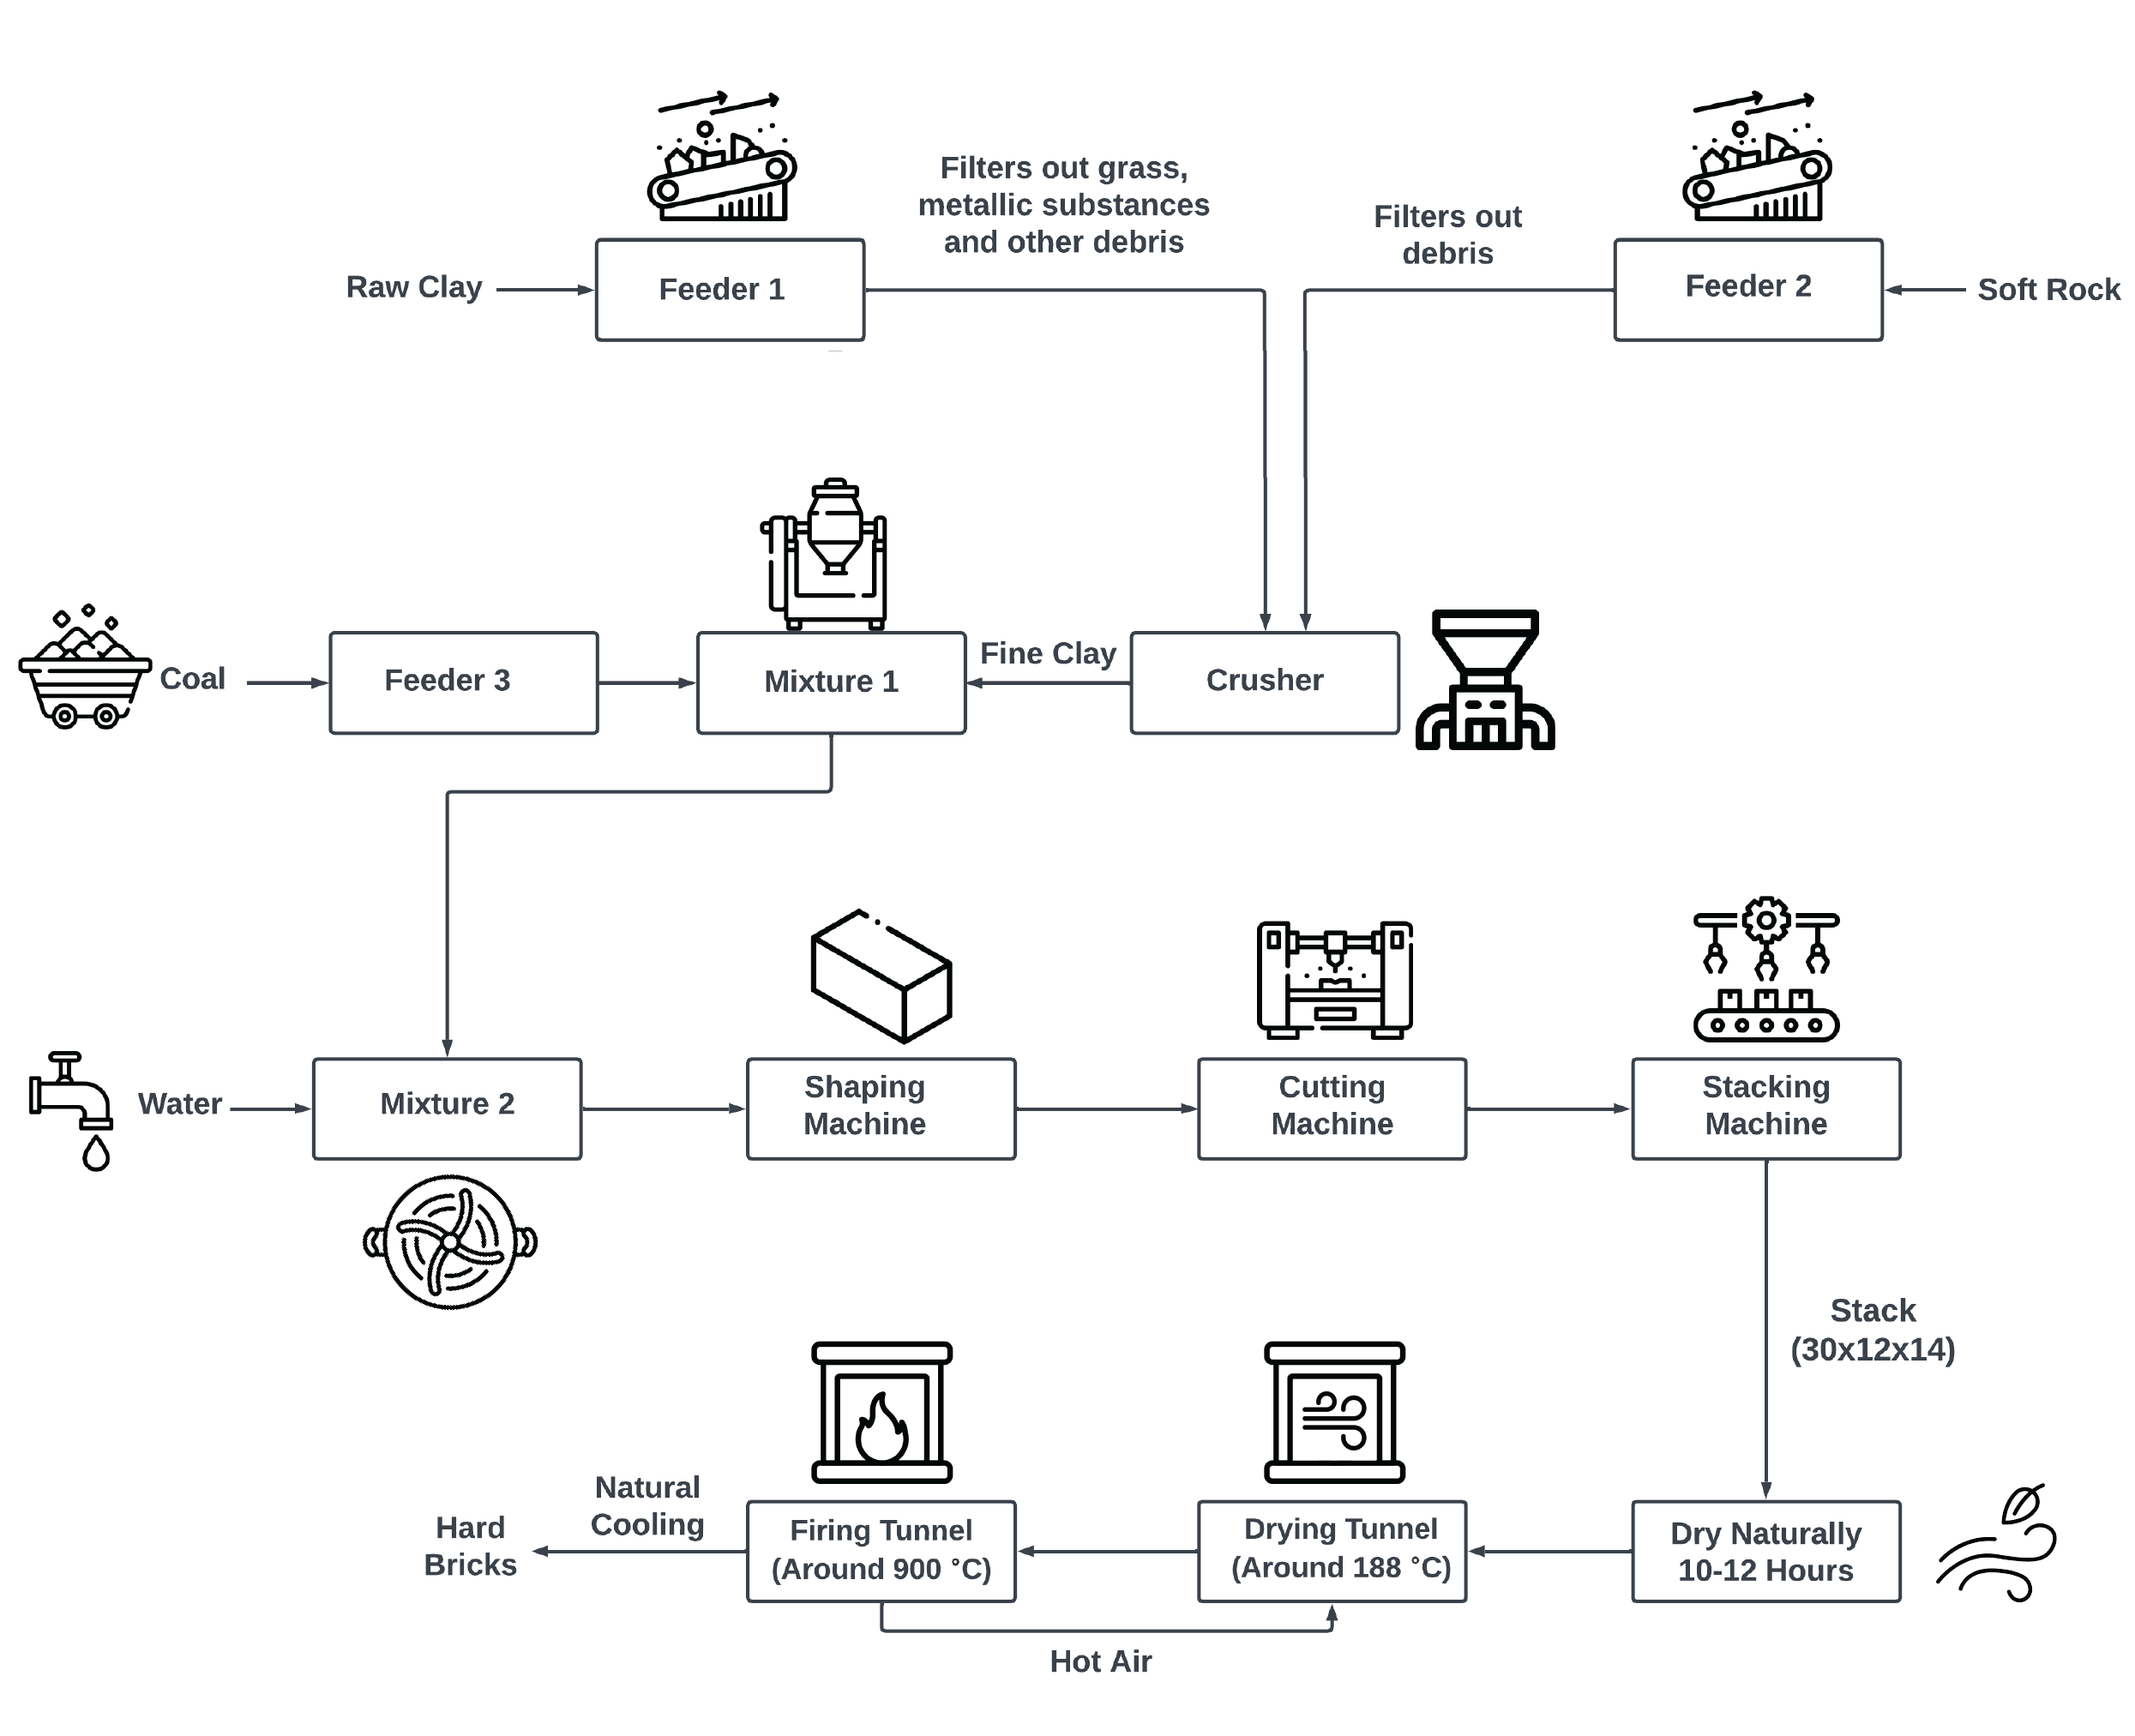
\includegraphics[width=1\textwidth]{img/block diagram.png}
  \caption{Block diagram for brick manufacture process}
\end{figure}

\subsection{Process Flow for Brick Manufacture}
% Detailed explanation of the brick manufacturing process flow.
\newpage
\section{Recommendations of the System}
% Recommendations for improving the brick manufacturing process.


\subsection{For Packaging of Bricks}
% Recommendations related to brick packaging.

\section{Discussion and Conclusion}
% Your discussion and conclusion about the brick factory case study.

\section{Photo Gallery}
% Insert your photo gallery here.

\section{References}
% Your references go here.

\end{document}